Este capítulo visa fornecer uma visão abrangente das etapas metodológicas empreendidas, desde a coleta de dados, passando pela implementação prática dos algoritmos utilizados e atigindo como objetivo o produto final do trabalho. A pesquisa foi elaborada para conduzir um breve estudo e avaliação sobre os modelos de aprendizado de máquina em evidência na literatura, objetivando ao fim desse processo, obter um mapeamento das regiões mais suscetíveis a incêndios florestais. Dessa forma, a proposta é utilizar alguns destes modelos e observar a efetividade de cada um deles na previsão das queimadas na Amazônia Legal, utilizando dados geoespaciais detalhados dos últimos dez anos (datado de 01/01/2014 à 01/01/2024), fornecidos pelo Programa Queimadas, do IBGE. O modelo que melhor se adaptar ao treinamento dos dados e assim apresentar os melhores resultados será utilizado para geração dos mapas preditores.

Para atingir os objetivos da pesquisa, foi adotada uma abordagem quali-quantitativa, onde o componente quantitativo envolve a análise estatística dos dados históricos e a aplicação dos diferentes modelos de aprendizado de máquina para prever incêndios. Além disso, foram utilizadas algumas métricas de desempenho já consolidadas na literatura para a análise dos modelos utilizados, fornecendo segurança na etapa de validação e garantindo uma pesquisa robusta e precisa das tendências de queimadas. A pesquisa também investiga as razões pelas quais alguns modelos superam outros em termos de desempenho. Isso envolve a análise dos parâmetros e características dos modelos, a interpretação dos fatores que influenciam suas previsões e a avaliação das variáveis ambientais e climáticas que afetam a ocorrência de incêndios. Esta etapa metodológica introduz alguns valores detalhados da Amazônia Legal, permitindo uma exploração aprofundada das características regionais e das dinâmicas de seus incêndios florestais. Isso posto, temos um projeto de caráter experimental e teórico que deve extrair como produto final desse conjunto de métodos e processos, um mapeamento objetivo das áreas mais vulneráveis a queimadas nos próximos *(quantidade de tempo)* anos e contribuir para a elaboração de mais trabalhos sobre o tema.

O fluxo do desenvolvimento do trabalho está disposto em seguida. Apesar da disposição de um fluxograma nos remeter à ideia de um trabalho parcial e linear, o treinamento de uma máquina que seja capaz de aprender consiste em uma prática de bastante retrocesso, onde as etapas se complementam e podem sofrer alterações para atingir resultados melhores. Entendendo isso, na figura 5, segue o fluxograma adotado neste projeto para treinar nossos modelos e criar um algoritmo eficaz:

\begin{figure}[ht]
    \centering
    \includegraphics[scale=0.5]{"imagens/fluxograma metodologia tcc.png"}
    \caption{Fluxograma metodológico para a implementação do sistema de previsão de queimadas - Fonte: O Próprio Autor}
\end{figure}

\section{Coleta de Dados}
Esta pesquisa contempla dados de boa parte do bioma amazônico, mais especificamente, a chamada Amazônia Legal. Esta parte do território brasileiro possui uma extensão de aproximadamente 5.015.146,008 km2, que representam cerca de 58,93\% do país e aproximadamente 60\% do território total do bioma Amazônia \cite{ibge04:mapabioma}. O foco principal da coleta de dados são os "Focos de Calor", característica atribuída à regiões potencialmente propícias ao início de incêndios. Inicialmente, foi realizada a busca por uma base de dados legítima advinda do programa, abrangendo os últimos dez anos de registros de queimadas no território do bioma Amazônia (2014-2024). A exportação dos dados foi feita de forma anual, em função das limitações da plataforma. Assim, o primeiro passo técnico consistiu em compilar todos esses dados em uma única tabela. Esse processo resultou em aproximadamente 1 milhão de focos de calor registrados, proporcionando uma base consistente para as análises futuras.

\subsection{Uso do Programa Queimadas}

A fonte de onde os dados foram retirados é o chamado ``Programa Queimadas'', um sistema que monitora e disponibiliza informações sobre focos de calor gratuitamente, com um repositório de dados relacionados à climatologia e geografia da região e que viabiliza, através de uma série de filtros e parâmetros, refinar a busca e extrair dados específicos conforme as necessidades de pesquisadores. Esta ferramenta foi fundamental para obter dados precisos e relevantes sobre os incêndios na Amazônia Legal. Ela faz parte de um projeto do Instituto Nacional de Pesquisas Espaciais (INPE). Além da sua extensa base de dados que cataloga informações desde o ano de 1998, é possível visualizar um mapa com os focos de calor observados diariamente e previsões de fogo para os próximos três dias.

Estas informações são atualizadas frequentemente a partir do monitoramento de diferentes modelos de satélites, que atuam para alimentar sua base de dados. Para este estudo, será utilizado o satélite de referência (Aquamarine) para obter as informações geoespaciais da região e popular a base de dados do projeto. Todas as características de um foco podem ser exportadas do sistema, no formato “comma-separated-values” (CSV), JavaScript Object Notation (Json), Keyhole Markup Language (KML) ou Shapefile. A amostragem coletada para o desenvolvimento deste modelo concebe dados de 01 de janeiro de 2014 até o dia 01 de janeiro de 2024, totalizando dez (10) anos de dados históricos e aproximadamente um milhão de linhas (mais precisamente novecentros e trinta e três mil, novecentros e cinquenta e quatro dados) com os focos de calor registrados pelo sistema, afim de obter um bom espectro de variações de clima, temperatura, entre outros atributos que foram mensurados ao longo desse período.

\subsection{Filtros, Escopo e Características da Coleta}

Como citado na seção anterior, o programa queimadas fornece filtros que facilitam a nossa abordagem. Disposto na Figura 6 e explicado nas próximas linhas do capítulo, para diminuir o escopo da coleta apenas às regiões que interessam ao projeto, foram utilizados os seguintes filtros:

\textbf{Localização:} O projeto abordou especificamente a Amazônia Legal, uma região que compreende a porção da floresta amazônica localizada no Brasil. Utilizando os filtros do Programa Queimadas, foi possível restringir a coleta a focos de calor dentro desta área geográfica, assegurando também que os dados fossem pertinentes ao bioma alvo do estudo posteriormente.

\textbf{Temporalidade:} Para garantir uma análise histórica e detectar padrões ao longo do tempo, foram coletados dados dos últimos dez anos. Esse período foi escolhido para proporcionar uma visão abrangente das variações e tendências na frequência e intensidade dos incêndios ao longo do tempo e também possibilitar ao modelo a compreensão de fatores de longo prazo, como as mudanças climáticas. Dada uma limitação na exportação do sistema, os dados foram coletados anualmente.

\textbf{Bioma:} O foco foi restrito ao bioma amazônico, o que exclui outros biomas brasileiros que poderiam diluir a análise e introduzir variáveis que não são relevantes para a previsão de incêndios na Amazônia Legal.

Utilizando essa base de exportação de dados para todos os anos (Figura 6), foram obtidos arquivos que compreendem os últimos dez anos de focos de calor da Amazônia. Cada um destes focos possui uma série de características, que variam de acordo com a época e a região identificada. A exportação dos dados fornece os seguintes atributos, que são úteis para análise e treinamento do nosso modelo:

Latitude e Longitude: Coordenadas geográficas que permitem a localização precisa dos focos, importantes para o mapeamento das incidências;
Data e Hora: Marcação temporal dos eventos, essencial para análise de tendências e padrões sazonais;
Satélite: Informação sobre o satélite que detectou o foco de calor, fornecendo detalhes sobre a tecnologia de monitoramento utilizada;
Município, Estado e País: Dados geográficos que permitem uma análise mais granular e contextualizada;
Número de Dias Sem Chuva e Precipitação: Variáveis meteorológicas que são relevantes para entender as condições que podem favorecer a ocorrência de incêndios;
Risco de Fogo: Avaliação do risco de fogo associada a cada foco, crucial para entender a gravidade e potencial dos eventos;
Bioma e FRP (Fire Radiative Power): Dados sobre o bioma específico e a intensidade de radiação emitida por fogo na região, fornecendo uma visão detalhada sobre a severidade dos incêndios. Um detalhe importante é que os dados de FRP só passaram a ser coletados a partir de 2018, portanto este atributo não consta nos focos de calor anteriores, dos anos de 2014 a 2017;
Abaixo, na figura 6, está disposta a interface de exportação de dados do Programa Queimadas:

\begin{figure}[ht]
    \centering
    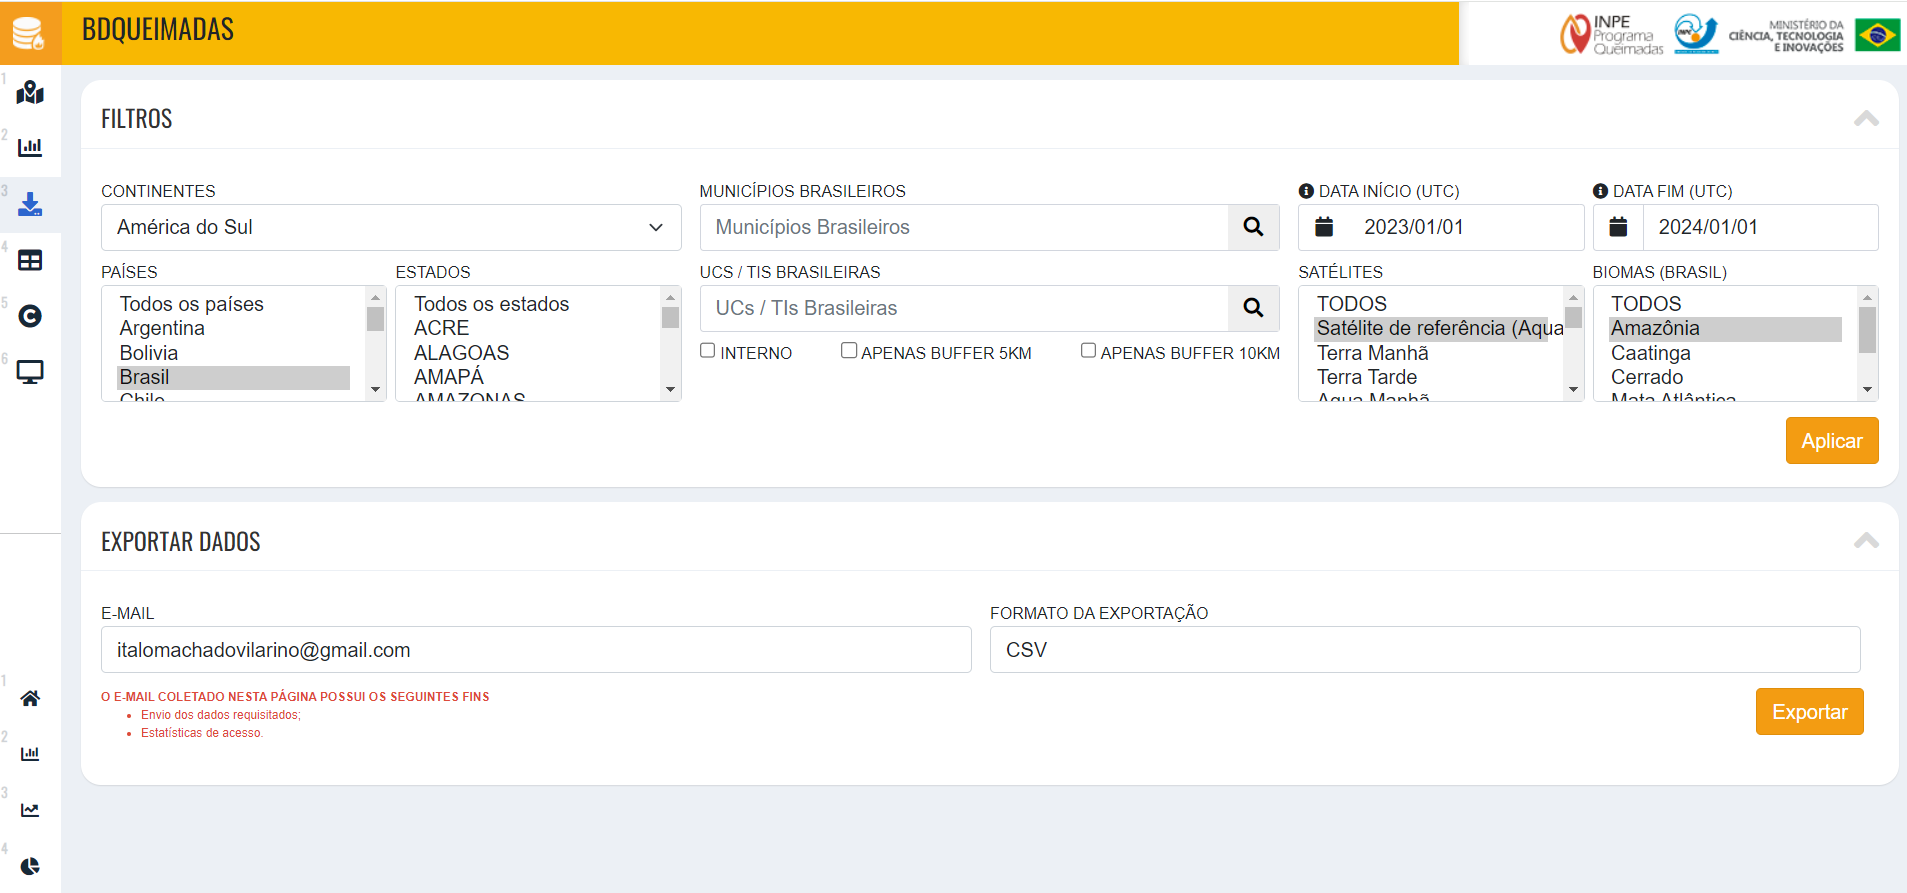
\includegraphics[scale=0.4]{imagens/Programa Queimadas-2.png}
    \caption{Interface de exportação de dados do Programa Queimadas - Fonte: IBGE}
\end{figure}

Com a base de dados obtida, o próximo passo realizado é o tratamento e normalização desses dados, para prepará-los para modelagem e análise preditiva.

\subsection{Enriquecimento via APIs externas (NASA POWER e NASA FIRMS)}
\label{subsec:metod_apis_externas}

Além do Programa Queimadas, duas APIs externas são consultadas para enriquecer o conjunto de dados:

\paragraph{NASA POWER (\emph{Prediction of Worldwide Energy Resources})~\cite{nasapower}.} Serve reanálise climática global em resolução de \(0{,}5^\circ \times 0{,}625^\circ\) com latência diária. Foi utilizada para extrair a variável RH2M (umidade relativa a 2~m), reconhecida na literatura como preditor relevante de fogo. A integração foi feita via \texttt{scripts/enriquecer\_dados\_umidade.py}, com \emph{cache} em disco, retomada após interrupção e respeito ao limite de taxa (\(\approx 32\)~requisições/min com duas chaves de API). Pela alta latência de enriquecimento total (\(\approx 16\)~dias para \num{755711} requisições únicas), o projeto adotou estratégia complementar: \num{170465} registros foram efetivamente enriquecidos (\(\approx \SI{18,3}{\percent}\) da base) e os \num{763489} restantes foram imputados via \emph{pseudo-labeling} com LightGBM \emph{regressor} (\(R^2 = 0{,}933\) em \emph{holdout} --- Seção~\ref{sec:metodologia_pseudo_label}).

\paragraph{NASA FIRMS (\emph{Fire Information for Resource Management System})~\cite{nasafirms}.} Serve detecções ativas de fogo em quase-tempo-real, com FRP (\emph{Fire Radiative Power}) por píxel para os sensores VIIRS e MODIS. É consultada em \textbf{tempo de inferência} pelo aplicativo web (Seção~\ref{sec:metod_app_web}) para incrementar a \emph{feature} \texttt{FRP} com observações dos últimos 7~dias na vizinhança do ponto consultado.

\section{Tecnologias, Bibliotecas e Ferramentas}

Este projeto foi desenvolvido utilizando a linguagem de programação \textbf{Python 3.12}, amplamente reconhecida por sua sintaxe concisa e rica biblioteca de pacotes, particularmente úteis para \textbf{ciência de dados} e \textbf{aprendizado de máquina}. As bibliotecas e ferramentas abaixo descritas foram essenciais para o \textbf{pré-processamento dos dados}, \textbf{análise preditiva} e \textbf{treinamento dos modelos}:

\begin{itemize}
    \item \textbf{Pandas}~\cite{mckinney2010data}: Utilizada para manipulação e análise de dados. A biblioteca fornece estruturas de dados eficientes, como os \textbf{DataFrames}, que facilitaram a importação, limpeza, transformação e exploração dos conjuntos de dados. Foi essencial para a organização e filtragem das informações, além de possibilitar a aplicação de operações vetorizadas nas variáveis numéricas e categóricas.

    \item \textbf{NumPy}~\cite{harris2020numpy}: Empregada para operações numéricas e manipulação de arrays. Como base para operações matemáticas e estatísticas em Python, a biblioteca \textbf{NumPy} proporcionou funções de alto desempenho para manipulação de dados, especialmente nas transformações numéricas aplicadas aos dados do projeto.

    \item \textbf{Scikit-Learn}~\cite{pedregosa2011scikit}: Esta biblioteca é a espinha dorsal do aprendizado de máquina em Python. Ela oferece uma ampla gama de ferramentas para pré-processamento de dados, seleção de modelos, avaliação de desempenho e implementação de algoritmos de aprendizado supervisionado e não supervisionado. No contexto deste projeto, as seguintes funcionalidades se destacaram:
    \begin{itemize}
        \item \textbf{Pipeline}: Utilizada para criar um fluxo de trabalho eficiente, encadeando as etapas de pré-processamento e modelagem em uma única estrutura. Essa abordagem facilitou o treinamento e a avaliação dos modelos de forma modular e repetível.

        \item \textbf{SimpleImputer}: Responsável pela imputação de valores ausentes. Essa ferramenta foi fundamental para preencher lacunas nos dados, utilizando estratégias como a mediana ou a moda, dependendo da natureza da variável.

        \item \textbf{StandardScaler}: Aplicada para a padronização das variáveis numéricas. Essa técnica garantiu que os dados estivessem na mesma escala, o que é crucial para melhorar a performance de muitos algoritmos de aprendizado de máquina, especialmente os baseados em distâncias e gradientes.

        \item \textbf{OneHotEncoder}: Utilizada para a codificação de variáveis categóricas, permitindo a conversão de dados categóricos em um formato binário adequado para a alimentação de modelos de aprendizado de máquina.

        \item \textbf{ColumnTransformer}: Facilitou a aplicação simultânea de diferentes transformações para diferentes grupos de atributos, permitindo a separação clara entre as variáveis numéricas e categóricas, o que otimizou o pré-processamento dos dados.
    \end{itemize}

    \item \textbf{Matplotlib} e \textbf{Seaborn}: Ferramentas poderosas para visualização de dados. Ambas as bibliotecas foram utilizadas para criar gráficos informativos e intuitivos, ajudando a identificar padrões, tendências e relações entre variáveis. O uso de gráficos de dispersão, histogramas e heatmaps foi fundamental para a análise exploratória dos dados e para a avaliação das previsões dos modelos de aprendizado de máquina.
\end{itemize}

Além dessas ferramentas, o projeto também utilizou outras bibliotecas complementares, como \textbf{Joblib}, para a serialização e armazenamento dos modelos treinados, e \textbf{Geopy}, para geocodificação de municípios, permitindo a criação de um mapa de risco de incêndios florestais na região da Amazônia.

\medskip
\noindent
Em complemento, o \emph{pipeline} atual incorpora também:

\begin{itemize}
  \item \textbf{XGBoost} (\texttt{xgboost})~\cite{chen2016xgboost}, \textbf{LightGBM} (\texttt{lightgbm})~\cite{ke2017lightgbm} e \textbf{CatBoost} (\texttt{catboost==1.2.10})~\cite{prokhorenkova2018catboost} --- modelos de \emph{gradient boosting} usados como classificadores autônomos e como \emph{base learners} dos \emph{ensembles}.
  \item \textbf{Imbalanced-learn} (\texttt{imblearn})~\cite{lemaitre2017imbalanced} --- implementação do SMOTE para a variante \texttt{random\_forest\_smote}.
  \item \textbf{Optuna} (\texttt{optuna})~\cite{akiba2019optuna} --- otimização bayesiana de hiperparâmetros via TPE.
  \item \textbf{SHAP} (\texttt{shap}) --- interpretabilidade local e global via \texttt{TreeExplainer}~\cite{lundberg2017unified,lundberg2020local}.
  \item \textbf{Flask} (\texttt{flask}) --- servidor web para a aplicação interativa.
  \item \textbf{Folium} (\texttt{folium})~\cite{folium} --- visualização cartográfica baseada em \emph{Leaflet}~\cite{leafletjs} integrada à renderização do Flask.
  \item \textbf{Geopandas} (\texttt{geopandas})~\cite{geopandas} e \textbf{Shapely} (\texttt{shapely}) --- manipulação de geometrias e do \emph{shapefile} da Amazônia Legal~\cite{ibgeamazonia2024}.
  \item \textbf{Requests} (\texttt{requests}) --- chamadas HTTP às APIs NASA POWER e NASA FIRMS.
\end{itemize}

\section{Pré-processamento dos dados}
\label{sec:metodologia_pre_processamento}

A primeira etapa técnica e prática do projeto foi o pré-tratamento dos dados. De maneira geral, as informações extraídas do Programa Queimadas mostraram-se bastante consistentes. No entanto, para assegurar a qualidade e a relevância dos dados em sua totalidade, essa fase é essencial para qualquer análise preditiva. O processo de pré-tratamento envolveu a aplicação de diversas técnicas descritas na fundamentação teórica, visando garantir que os dados estivessem prontos para as análises subsequentes.

\subsection{Carregamento dos Dados}

A função \texttt{carregar\_csv()} foi responsável por carregar o conjunto de dados a partir de um arquivo CSV. Caso o arquivo não seja encontrado no caminho especificado, a função gera um erro indicando a ausência do arquivo. Uma vez carregado, o arquivo é lido como um \texttt{DataFrame} utilizando a biblioteca \texttt{pandas}. O caminho para o arquivo CSV foi especificado como sendo relativo ao diretório do projeto.

\subsection{Limpeza dos Dados}

Após o carregamento dos dados, a função \texttt{limpar\_dados()} realiza o processo de limpeza e tratamento dos dados. Entre as principais etapas dessa função, destacam-se:

\begin{itemize}
    \item \textbf{Remoção de Colunas Irrelevantes:} As colunas \texttt{Satelite}, \texttt{Pais} e \texttt{Bioma} são removidas, uma vez que não são relevantes para a análise do risco de queimadas.
    \item \textbf{Substituição de Valores Inválidos:} Valores de \texttt{-999} são substituídos por \texttt{NaN}, indicando dados ausentes ou corrompidos.
    \item \textbf{Filtragem de Linhas com Dados Inválidos:} Linhas com valores inválidos ou nulos na coluna \texttt{RiscoFogo} são removidas, garantindo que os dados utilizados na análise contenham apenas informações válidas.
\end{itemize}

Durante a execução desta função, a quantidade de registros que atendem a essa condição de validade (\texttt{RiscoFogo}) é reportada, proporcionando uma visão sobre a quantidade de dados descartados nesse processo.

\subsection{Classificação do Risco de Queimadas}

Após a limpeza dos dados, a função \texttt{classificar\_risco()} é responsável por categorizar o risco de queimadas com base nos valores da coluna \texttt{RiscoFogo}. A classificação é realizada utilizando os quantis da distribuição dessa variável, dividindo os dados em três categorias:

\begin{itemize}
    \item \textbf{Muito Alto:} Valores de \texttt{RiscoFogo} acima do quantil superior (66\%).
    \item \textbf{Moderado:} Valores de \texttt{RiscoFogo} entre os quantis inferior (33\%) e superior (66\%).
    \item \textbf{Baixo:} Valores de \texttt{RiscoFogo} abaixo do quantil inferior (33\%).
\end{itemize}

Essas categorias são atribuídas a uma nova coluna chamada \texttt{RiscoClassificado}, que é utilizada como variável alvo (\texttt{y}) para o treinamento dos modelos de aprendizado de máquina.

\subsection{Definição das Características e Variáveis}

A função \texttt{carregar\_dados()} organiza os dados em variáveis preditoras (\texttt{X}) e variável alvo (\texttt{y}):

\begin{itemize}
    \item \textbf{Variáveis Preditivas (\texttt{X}):} Incluem as colunas numéricas (\texttt{DiaSemChuva}, \texttt{Precipitacao}, \texttt{Latitude}, \texttt{Longitude}, \texttt{FRP}, \texttt{Ano}, \texttt{Mes}, \texttt{Dia}, \texttt{Hora}) e as variáveis categóricas (\texttt{Estado}, \texttt{Municipio}).
    \item \textbf{Variável Alvo (\texttt{y}):} A coluna \texttt{RiscoClassificado}, que representa a classificação do risco de queimadas.
\end{itemize}

\subsection{Pré-processamento dos Dados}

O pré-processamento dos dados foi realizado através da classe \texttt{PreProcessor}, que aplica transformações adequadas tanto para variáveis numéricas quanto para variáveis categóricas. O pré-processamento foi dividido nas seguintes etapas:

\begin{itemize}
    \item \textbf{Transformação de Variáveis Numéricas:} As variáveis numéricas (\texttt{DiaSemChuva}, \texttt{Precipitacao}, \texttt{Latitude}, \texttt{Longitude}, \texttt{FRP}, \texttt{Ano}, \texttt{Mes}, \texttt{Dia}, \texttt{Hora}) passaram por duas operações: imputação de valores ausentes utilizando a mediana e normalização utilizando o \texttt{StandardScaler}.
    \item \textbf{Transformação de Variáveis Categóricas:} As variáveis categóricas (\texttt{Estado}, \texttt{Municipio}) foram tratadas com imputação de valores ausentes pela moda (valor mais frequente) e transformação em variáveis numéricas através de \texttt{OneHotEncoder}, que cria variáveis binárias para cada categoria.
\end{itemize}

A transformação dos dados foi realizada utilizando um \texttt{ColumnTransformer}, que aplica as transformações apropriadas para cada tipo de variável, permitindo que o modelo trabalhe com dados prontos para a análise.

A classe \texttt{PreProcessor} também oferece métodos para \texttt{fit} e \texttt{transform} dos dados, além de retornar um \texttt{DataFrame} com as variáveis transformadas. Essa etapa é crucial para garantir que os dados estejam em um formato adequado para o treinamento dos modelos.

\subsection{Fluxo Completo de Carregamento e Pré-processamento}

O fluxo de carregamento e pré-processamento dos dados é executado como segue:

\begin{enumerate}
    \item Carregamento dos dados do arquivo CSV.
    \item Limpeza dos dados, removendo colunas irrelevantes e tratando valores ausentes ou inválidos.
    \item Classificação do risco de queimadas com base na variável \texttt{RiscoFogo}.
    \item Definição das variáveis preditoras (\texttt{X}) e alvo (\texttt{y}).
    \item Aplicação do pré-processamento, incluindo imputação e normalização das variáveis.
\end{enumerate}

Esse processo assegura que os dados utilizados para o treinamento dos modelos estejam limpos, estruturados e prontos para análise preditiva.

\subsection{Engenharia de \emph{features} físico-climáticas (Tier 1)}
\label{subsec:metod_features_tier1}

Em complemento às nove \emph{features} originais do Programa Queimadas, foram derivadas \textbf{24~\emph{features} físico-climáticas avançadas} (Tier~1), agrupadas em sete camadas (implementação em \texttt{scripts/features\_avancadas.py}). A Tabela~\ref{tab:metod_tier1} resume as camadas com a justificativa bibliográfica de cada uma.

\begin{table}[h]
\centering
\caption{Camadas Tier~1 de \emph{features} físico-climáticas adicionadas ao \emph{dataset}.}
\label{tab:metod_tier1}
\small
\begin{tabular}{clp{6cm}l}
\toprule
\textbf{\#} & \textbf{Camada} & \textbf{\emph{Features}} & \textbf{Justificativa} \\
\midrule
1 & Médias móveis estendidas & \texttt{Precipitacao\_ma14/30/90}, \texttt{DiaSemChuva\_ma14/30/90} & \emph{Fuel moisture lag}~\cite{seager2015climatology} \\
2 & Precipitação acumulada & \texttt{Precipitacao\_acum\_30/90/180/365d} & \cite{seager2015climatology} \\
3 & SPI & \texttt{SPI\_1m}, \texttt{SPI\_3m}, \texttt{SPI\_6m} & \cite{mckee1993spi,npjhazards2025fire} \\
4 & Anomalia de precipitação & \texttt{Anomalia\_Precipitacao}, \texttt{Anomalia\_Precipitacao\_rel} & \cite{forests2024cerradoamazon} \\
5 & KBDI, VPD, De Martonne & \texttt{Temp\_Climatologica}, \texttt{KBDI\_proxy}, \texttt{VPD\_proxy}, \texttt{Aridez\_DeMartonne} & \cite{keetch1968drought,seager2015climatology,demartonne1926aridity,forests2024cerradoamazon} \\
6 & Histórico estendido de incêndios & \texttt{Incendios\_Ultimos\_90/180/365\_Dias}, \texttt{Media\_FRP\_Celula\_30d} & \cite{cheerala2025probabilistic} \\
7 & Estação seca acumulada & \texttt{Dias\_Secos\_90d} & \emph{Canadian Drought Code} (FWI) \\
\bottomrule
\end{tabular}
\end{table}

A granularidade espacial das camadas 1, 2, 6, 7 e do SPI usa \textbf{células de \(0{,}25^\circ\)} (\(\approx \SI{27}{\km}\)), o que evita colapso das janelas temporais que ocorreria com agrupamento por coordenadas literais (cada foco é um ponto único). A \emph{climatologia} de temperatura provém de uma tabela estática de médias mensais por estado, aproximada a partir das Normais Climatológicas do INMET 1981--2010~\cite{inmetnormais}. O CSV final \texttt{base\_de\_dados\_enriquecido.csv} contém \num{924306} linhas e 46~colunas, com tempo total de geração de \(\approx \SI{40}{\second}\) sobre os \num{933954} registros brutos.

\subsection{Calibração de probabilidades}
\label{subsec:metod_calibracao}

A predição padrão dos modelos retorna escores não-calibrados. Para que a saída do modelo seja interpretável como ``\(P(\text{classe} \mid \text{features}) = 0{,}73\)'', aplicou-se \texttt{CalibratedClassifierCV(method='isotonic', cv=3)} aos modelos do \emph{ensemble} final. A calibração isotônica~\cite{zadrozny2002transforming} ajusta uma função monotônica não-paramétrica entre escores brutos e probabilidades empíricas, sem assumir forma sigmoide --- escolha defensável dada a natureza não linear dos GBMs envolvidos.

\section{Treinamento dos Modelos de Previsão}
\label{sec:metod_treinamento}

Neste ponto, todos os algoritmos utilizaram a mesma \emph{pipeline}, garantindo que os dados fossem preparados de maneira consistente para os processos de treinamento e teste. O objetivo foi comparar os resultados gerados por cada modelo em um cenário base comum, assegurando que não houvesse qualquer tipo de viés, exceto aqueles originados exclusivamente pelo desempenho de cada algoritmo. A partir de um conjunto de dados previamente processados, foram aplicados algoritmos de classificação para identificar as áreas mais suscetíveis a queimadas com base em atributos climáticos, topográficos e históricos.

O treinamento dos modelos foi realizado utilizando a biblioteca \texttt{scikit-learn}~\cite{pedregosa2011scikit}, complementada por \texttt{xgboost}~\cite{chen2016xgboost}, \texttt{lightgbm}~\cite{ke2017lightgbm}, \texttt{catboost}~\cite{prokhorenkova2018catboost}, \texttt{optuna}~\cite{akiba2019optuna} e \texttt{imbalanced-learn}~\cite{lemaitre2017imbalanced}.

\subsection{Divisão dos dados e construção do \emph{pipeline}}

O conjunto de dados foi dividido em treino (\SI{80}{\percent}) e teste (\SI{20}{\percent}) utilizando \texttt{train\_test\_split(stratify=y, random\_state=42)}, preservando a distribuição das três classes em ambos os subconjuntos. Os metadados do \emph{split} (\texttt{random\_state}, \texttt{test\_size}, estratificação) ficam persistidos em \texttt{modelos/split\_metadata.json} para garantir reprodutibilidade. O conjunto de teste contém \num{184862} observações.

O \emph{pipeline} de processamento foi implementado via \texttt{sklearn.pipeline.Pipeline}, composto por:

\begin{enumerate}
  \item \texttt{ColumnTransformer} --- aplica \texttt{SimpleImputer(strategy='median')} + \texttt{StandardScaler} às \emph{features} numéricas e \texttt{SimpleImputer(strategy='most\_frequent')} + \texttt{OneHotEncoder} às \emph{features} categóricas.
  \item \texttt{CalibratedClassifierCV(method='isotonic', cv=3)} --- envolve o classificador final para garantir calibração das probabilidades.
  \item \textbf{Estimador} --- variável conforme o modelo avaliado.
\end{enumerate}

\subsection{Modelos avaliados}

Oito abordagens foram comparadas no mesmo conjunto de treino/teste:

\begin{enumerate}
  \item \textbf{Regressão Logística balanceada} --- \texttt{class\_weight='balanced'}, hiperparâmetros otimizados via Optuna (\texttt{C=12.43, max\_iter=4768}).
  \item \textbf{SGDClassifier} --- perda logística, \emph{online learning}; \emph{baseline} simples original do projeto.
  \item \textbf{Random Forest com SMOTE}~\cite{chawla2002smote} --- variante para tratamento de desbalanceamento amostral.
  \item \textbf{Random Forest balanceado otimizado}~\cite{breiman2001random} --- \texttt{class\_weight='balanced'}, Optuna (15 \emph{trials}, 3-\emph{fold} CV, \(\text{F}_1\)-macro): \texttt{n\_estimators=346, max\_depth=25, min\_samples\_split=3, max\_features='sqrt'}.
  \item \textbf{XGBoost otimizado}~\cite{chen2016xgboost} --- Optuna (15 \emph{trials}, 3-\emph{fold} CV, \(\text{F}_1\)-macro, \emph{subsample} de 250\,k): \texttt{n\_estimators=346, learning\_rate=0.073, max\_depth=14, subsample=0.74, colsample\_bytree=0.93, gamma=0.03}.
  \item \textbf{LightGBM otimizado}~\cite{ke2017lightgbm} --- Optuna (15 \emph{trials}, \(\text{F}_1\)-macro): \texttt{n\_estimators=683, learning\_rate=0.066, num\_leaves=204, min\_child\_samples=24, subsample=0.78, colsample\_bytree=0.77}.
  \item \textbf{CatBoost}~\cite{prokhorenkova2018catboost} --- \texttt{iterations=1000, learning\_rate=0.05, depth=8, auto\_class\_weights='Balanced'}.
  \item \textbf{Ensemble Voting Soft} --- média das probabilidades calibradas de RF, LR, XGBoost, LightGBM e CatBoost.
  \item \textbf{Ensemble Stacking}~\cite{wolpert1992stacked} --- RF, LR, XGBoost, LightGBM e CatBoost como \emph{base learners}; \texttt{GradientBoostingClassifier}~\cite{friedman2001greedy} como meta-classificador (\texttt{n\_estimators=200, max\_depth=3, learning\_rate=0.1}). Esta é a configuração final adotada (\texttt{ensemble\_stacking\_gbm}).
\end{enumerate}

Todos os modelos foram salvos via \texttt{joblib.dump()} em arquivos \texttt{.pkl} no diretório \texttt{modelos/}. Os hiperparâmetros otimizados via Optuna ficam persistidos em \texttt{modelos/relatorios/optuna\_*.json}.

\subsection{Tempo de treinamento}

A Tabela~\ref{tab:metod_tempos} apresenta o tempo de treinamento de cada abordagem em ambiente CPU com 8~núcleos e \SI{16}{\giga\byte} de RAM.

\begin{table}[h]
\centering
\caption{Tempo de treinamento por modelo.}
\label{tab:metod_tempos}
\small
\begin{tabular}{lr}
\toprule
\textbf{Modelo} & \textbf{Tempo (segundos)} \\
\midrule
Regressão Logística balanceada & 25 \\
SGDClassifier                  & 8 \\
Random Forest + SMOTE          & 480 \\
Random Forest balanceado (Optuna) & 1\,100 \\
XGBoost (Optuna, 250k \emph{subsample}) & 540 \\
LightGBM (Optuna, 250k \emph{subsample}) & 290 \\
CatBoost                       & 410 \\
Ensemble Voting Soft           & 2\,360 (soma dos \emph{base learners} + agregação) \\
\textbf{Ensemble Stacking GBM} & \textbf{5\,100 (\(\approx\) 85~min)} \\
\bottomrule
\end{tabular}
\end{table}

\section{Avaliação dos Modelos de Previsão}
\label{sec:metod_avaliacao}

A avaliação foi realizada sobre o conjunto de teste de \num{184862} observações. Quatro componentes complementares foram considerados: métricas tradicionais (Seção~\ref{subsec:metod_metricas}), interpretabilidade (Seção~\ref{subsec:metod_interpretabilidade}), ajuste multi-classe de limiares (Seção~\ref{subsec:metod_thresholds}) e validação temporal estrita (Seção~\ref{subsec:metod_validacao_temporal}).

\subsection{Métricas utilizadas}
\label{subsec:metod_metricas}

\begin{itemize}
  \item \textbf{Acurácia global} --- fração de predições corretas (\texttt{accuracy\_score}).
  \item \textbf{\(\text{F}_1\) por classe e \(\text{F}_1\)-macro} --- \texttt{f1\_score(average='macro')}. A \(\text{F}_1\)-macro é a média não ponderada entre as três classes; é a métrica primária por ser robusta a desbalanceamento.
  \item \textbf{Precisão e revocação por classe} --- via \texttt{classification\_report}.
  \item \textbf{Matriz de confusão normalizada} --- \texttt{confusion\_matrix(normalize='true')}.
  \item \textbf{Confiança média e distribuição} --- média e histograma de \(\max\) de \texttt{predict\_proba(X\_test)}.
  \item \textbf{Curva de calibração} --- \texttt{calibration\_curve}, para confirmar que a probabilidade predita corresponde à frequência empírica observada.
\end{itemize}

\subsection{Análise de interpretabilidade}
\label{subsec:metod_interpretabilidade}

Duas técnicas complementares são aplicadas para identificar as \emph{features} mais relevantes:

\paragraph{SHAP por classe via Random Forest leve \emph{proxy}~\cite{lundberg2017unified,lundberg2020local}.} O \texttt{TreeExplainer} aplicado ao \emph{Stacking GBM} final e ao RF Optuna produtivo demanda mais de \num{2}\,\text{GiB} por classe em CPU pós-OHE. Como solução cientificamente defensável~\cite{lundberg2020local}, treina-se um Random Forest \emph{compacto} (100 árvores, \texttt{max\_depth=12}, \texttt{class\_weight='balanced'}, \num{60000} amostras de treino) como \emph{proxy interpretativo}. O script \texttt{scripts/analise\_shap\_rf\_leve.py} aplica \texttt{shap.TreeExplainer} sobre 500 amostras de teste e exporta as importâncias médias absolutas por classe em \texttt{modelos/relatorios/shap\_per\_class.json}.

\paragraph{\emph{Permutation Importance}~\cite{breiman2001random,fisher2019all}.} Aplicada diretamente sobre o \texttt{ensemble\_stacking\_gbm} em produção (5\,000 amostras de teste, três repetições, \emph{seed}=42). Para cada \emph{feature}, calcula-se a queda em \(\text{F}_1\) por classe e em \(\text{F}_1\)-macro quando os valores são permutados aleatoriamente. Diferentemente da importância Gini/MDI, é \emph{model-agnostic} e \textbf{não tendenciosa} para \emph{features} de alta cardinalidade~\cite{strobl2007bias} --- característica relevante dado o OHE de \texttt{Municipio} (542 categorias). A saída fica em \texttt{modelos/relatorios/permutation\_importance\_por\_classe.json}.

\subsection{Ajuste multi-classe de limiares de decisão}
\label{subsec:metod_thresholds}

A predição padrão usa \texttt{argmax} sobre as probabilidades calibradas. Embora maximize \(P(\text{classe} \mid x)\), penaliza a classe \emph{Moderado} --- fronteira ambígua entre \emph{Baixo} e \emph{Muito Alto}~\cite{he2009learning}. O procedimento implementado em \texttt{scripts/ajustar\_threshold.py} varre uma grade de pares (\texttt{thr\_Moderado}, \texttt{thr\_Muito\_Alto}) \(\in \{0{,}30; 0{,}35; \ldots; 0{,}55\}^2\) (36 combinações), com critério primário \(\text{F}_1\)-macro e secundário \(\text{F}_1\)-Moderado. Os limiares finais são persistidos em \texttt{modelos/prediction\_thresholds.json} e aplicados em \emph{runtime} no aplicativo web via parâmetro \texttt{estrategia\_thresholds} do \emph{endpoint} \texttt{/api/predict}.

A lógica de decisão multi-classe em \emph{runtime} é:

\begin{verbatim}
se      P(Moderado)   >= thr_Moderado    -> classe = "Moderado"
senao se P(Muito Alto) >= thr_Muito_Alto -> classe = "Muito Alto"
senao                                    -> classe = "Baixo"
\end{verbatim}

\subsection{Validação temporal (\emph{rolling-origin})}
\label{subsec:metod_validacao_temporal}

Em complemento à validação no \emph{split} aleatório, foi implementado em \texttt{scripts/validacao\_temporal.py} um procedimento de \textbf{\emph{rolling-origin} por ano}~\cite{bergmeir2012cv}. Para cada ano \(Y \in \{2021, 2022, 2023\}\) (três últimos com massa suficiente), o modelo é treinado em \(\text{Ano} < Y\) (\emph{subsample} estratificado de \num{60000} amostras por \emph{fold} para o \emph{Stacking}, limite de memória do OHE denso de \texttt{Municipio}) e avaliado em \(\text{Ano} = Y\). Cobre o uso operacional realista: ``treine com o passado, prediga o ano seguinte''. O resultado é apresentado no Capítulo~\ref{cap:resultados}.

\section{Aplicação web interativa explicável}
\label{sec:metod_app_web}

Para tornar o modelo final utilizável e auditável por gestores ambientais, foi desenvolvida uma aplicação web (\texttt{scripts/app\_map\_interativo.py}) baseada em \emph{Flask} + \emph{Folium}~\cite{folium} + \emph{Leaflet}~\cite{leafletjs} que serve como interface explicável sobre o \emph{pipeline}. O usuário clica em qualquer ponto da Amazônia Legal e o sistema responde, em \(\approx 10\)--\SI{20}{\second}, com a predição classificada, acompanhada das 24~\emph{features} Tier~1 calculadas para o ponto, da explicação local das \emph{features} mais influentes e do contexto histórico comparativo.

\subsection{\emph{Pipeline} de predição pontual}

Como o aplicativo prediz \textbf{um único ponto isolado}, sem histórico temporal local, as \emph{features} Tier~1 que dependem de séries (SPI, acumulados longos, histórico estendido de focos) não podem ser calculadas em tempo real. Adota-se a estratégia de \textbf{\emph{lookup} espaço-sazonal} (\texttt{scripts/feature\_lookup.py}):

\begin{enumerate}
  \item Pré-cálculo das medianas das 24~\emph{features} Tier~1 do \emph{dataset} enriquecido, agregadas em três níveis de granularidade decrescente: \((\text{LatBin}~0{,}25^\circ, \text{LonBin}~0{,}25^\circ, \text{Mes})\), depois \((\text{Estado}, \text{Mes})\) e, por fim, \text{Mes} global.

  \item Para o ponto consultado, \emph{lookup} em cascata (do mais fino ao mais grosso) com tolerância de \(\pm 1\) célula.

  \item \emph{Features} físicas independentes de série temporal (\texttt{Temp\_Climatologica}, \texttt{KBDI\_proxy}, \texttt{VPD\_proxy}, \texttt{Aridez\_DeMartonne}, \texttt{Anomalia\_Precipitacao}) são recalculadas em tempo real com o clima NASA POWER atual e a climatologia local da precipitação --- o \emph{lookup} fornece apenas os ``blocos de construção'' históricos imutáveis.
\end{enumerate}

\subsection{Integração de dados em tempo real}

\begin{itemize}
  \item \textbf{Geocodificação reversa} via Nominatim/OpenStreetMap para extrair Estado e Município do clique.
  \item \textbf{Clima atual} via NASA POWER~\cite{nasapower} (precipitação, dias sem chuva, RH2M dos últimos 28~dias).
  \item \textbf{Focos ativos} via NASA FIRMS~\cite{nasafirms} para \texttt{FRP} dos últimos 7~dias no raio de \SI{10}{\km} do ponto.
\end{itemize}

\subsection{Explicabilidade local}

Em \emph{runtime}, \texttt{scripts/explainer.py} aproxima a contribuição de cada \emph{feature} como
\begin{equation}
\text{contrib}(f) = \text{importância}(f) \times \text{zscore}(f) \times \text{sinal\_físico}(f),
\end{equation}
onde \(\text{importância}(f)\) é carregada de \texttt{shap\_per\_class.json} (importância por classe predita, quando disponível) ou de \texttt{shap\_feature\_importance.json} (Gini global como \emph{fallback}); \(\text{zscore}(f)\) mede a anormalidade do valor no ponto em relação à distribuição global do \emph{dataset}; e \(\text{sinal\_físico}(f) \in \{-1, +1\}\) codifica o efeito esperado (por exemplo, \(+1\) para \texttt{Indice\_Seca}, \(-1\) para \texttt{Precipitacao\_ma90}). A predição é classificada como \emph{AUMENTA RISCO}, \emph{REDUZ RISCO} ou \emph{neutro}; o \emph{top-6 features} por \(|\text{contrib}|\) é exibido no painel lateral.

\subsection{Interface}

O \emph{front-end} é organizado em \textbf{seis \emph{cards}} dentro de um painel lateral de \SI{420}{px}:

\begin{enumerate}
  \item \textbf{Previsão} --- \emph{badge} com a classe, barras de probabilidade por classe, métricas do modelo, fonte do clima, granularidade do \emph{lookup} e \emph{trace} da decisão (\emph{argmax} \emph{vs.}\ \emph{thresholds} calibrados).
  \item \textbf{Por que esse risco?} --- \emph{top-6 features} com valor, faixa típica (\(p_{10}\)--\(p_{90}\) da distribuição global), \emph{z-score} e direção do impacto.
  \item \textbf{Dados climáticos atuais} --- precipitação, dias sem chuva, umidade NASA, temperatura climatológica, estação, período do dia.
  \item \textbf{Índices de seca e aridez} --- Índice de Seca, SPI 1m/3m/6m, KBDI \emph{proxy}, Aridez De Martonne, VPD \emph{proxy}, Dias\_Secos\_90d.
  \item \textbf{Precipitação acumulada e anomalia} --- acumulados 30/90/180/365~dias com narrativa textual comparando precipitação atual e a média histórica do município/mês.
  \item \textbf{Histórico de focos} --- focos NASA FIRMS em 7/30/90/180/365~dias, dias desde o último foco, FRP médio/máximo 7d, FRP no ponto agora.
\end{enumerate}

O mapa estático (versão original da Seção 4.6 do TCC~II) permanece disponível como artefato \emph{batch} (\texttt{scripts/gerar\_mapa.py}).

\section{Imputação de \emph{Umidade} via \emph{pseudo-labeling}}
\label{sec:metodologia_pseudo_label}

Como discutido na Seção~\ref{subsec:metod_apis_externas}, a integração via NASA POWER produziu \num{170465} linhas com \texttt{Umidade} real (\(\approx \SI{18,3}{\percent}\) da base). Para mitigar essa cobertura parcial sem aguardar 13~dias adicionais de enriquecimento, foi implementada a estratégia de \textbf{\emph{pseudo-labeling}}~\cite{lee2013pseudo}, com precedente recente em imputação climática~\cite{lopezgarcia2024spatiotemporal}. O \emph{script} \texttt{scripts/pseudo\_label\_umidade.py} executa as etapas:

\begin{enumerate}
  \item Treina um \textbf{LightGBM regressor}~\cite{ke2017lightgbm} sobre os \(\approx \num{170000}\) registros com \texttt{Umidade} real, usando 15~\emph{features} (precipitação, dias sem chuva, lat/lon, sazonalidade cíclica \texttt{Mes\_sin/cos}, histórico de fogo) --- \emph{features} que existem para todas as linhas, com ou sem \texttt{Umidade} real.

  \item Avalia o erro real em \emph{holdout} 20\%: \textbf{RMSE = \SI{4,33}{\percent} RH, MAE = \SI{3,19}{\percent} RH, \(R^2 = 0{,}933\)}. O \(R^2\) alto é cientificamente justificável: a umidade tem alta autocorrelação espaço-sazonal com as \emph{features} usadas --- lat/lon definem o regime de monção, mês define a estação seca/chuvosa, precipitação recente define o estado higroscópico do ar.

  \item Refit no \SI{100}{\percent} dos \emph{labels} reais e imputa os \num{763489} registros sem \emph{label} (\emph{clip} [5, 100]\%).

  \item Salva o \emph{dataset} enriquecido em \texttt{base\_de\_dados\_umidade\_pseudo.csv} com coluna auxiliar \texttt{Umidade\_origem} \(\in\) \{\texttt{nasa\_power}, \texttt{pseudo\_label\_lgbm}\} para auditoria.
\end{enumerate}

\paragraph{Status no \emph{pipeline} final.} O \emph{dataset} \texttt{base\_de\_dados\_umidade\_pseudo.csv} está disponível mas \textbf{não é usado nos números finais reportados} no Capítulo~\ref{cap:resultados}. Razão: incluir \texttt{Umidade} (pseudo-rotulada ou real) exigiria retreino completo do \texttt{ensemble\_stacking\_gbm} (\(\approx \SI{85}{\minute}\) CPU) + revalidação das \emph{thresholds} + revalidação temporal --- fora do orçamento computacional desta entrega. O artefato fica registrado como \textbf{etapa preparatória} para a sequência natural do trabalho. Cautela registrada: \emph{pseudo-labels} devem ser interpretados considerando potencial viés de confirmação~\cite{arazo2020pseudo}.

\section{Geração do Mapa de Risco com Previsões do Modelo}

A versão original do mapa de risco --- gerada em modo \emph{batch} sobre um conjunto pré-definido de pontos e exportada como arquivo HTML estático --- permanece disponível em \texttt{scripts/gerar\_mapa.py} como artefato histórico. A entrega operacional final do projeto, contudo, é a \textbf{aplicação web interativa} descrita na Seção~\ref{sec:metod_app_web}, em que o usuário aponta qualquer ponto da Amazônia Legal e recebe imediatamente predição, intervalo de confiança, explicação local e contexto climático/histórico --- tornando obsoleta a estratégia batch para uso prático e, em particular, eliminando o gargalo de geocodificação prévia. As bibliotecas envolvidas (\texttt{pandas}, \texttt{joblib}, \texttt{geopy}, \texttt{folium}, \texttt{webbrowser}) seguem em uso, agora orquestradas pelo servidor Flask.

\chapter{Resultados}
\label{cap:resultados}

